\documentclass{beamer}

\usepackage[T1]{fontenc}
\usepackage[brazil]{babel}
\usepackage[utf8]{inputenc}
\usepackage{graphicx}
\usepackage{textcomp}

% Add the citation package
\usepackage[alf,abnt-emphasize=bf]{abntex2cite}

% Choose the Inf theme
\usetheme{Inf}

% --- Title Information ---
\title[HIoT Data Security with MA-ABE]{A Hybrid Multi-Authority Attribute-Based Encryption Scheme For Securing HIoT Data}
\author{Felipe de Almeida Graeff}
\institute{Instituto de Informática --- UFRGS \\ \vspace{0.5cm} Advisor: Prof. Dr. Jéferson Campos Nobre \\ Co-advisor: M.Sc Laura Rodrigues Soares}
\date{8 de julho de 2025}

\begin{document}

% --- Title Page ---
\begin{frame}[plain]
\titlepage
\end{frame}

% --- Agenda ---
\begin{frame}
\frametitle{Agenda}
\tableofcontents
\end{frame}

% --- Introduction ---
\section{Introduction}

\begin{frame}
\frametitle{Background}
\begin{itemize}
\item \citeonline{laura2023} proposed a decentralized architecture for the Health Internet of Things (HIoT) using decentralized storage and blockchain technologies.
\item Their work lacks a robust cryptographic solution to ensure data confidentiality, data ownership, access control, and privacy.
\item We extend their framework by proposing a hybrid cryptographic approach to enhance the security of the system and enable fine-grained access control based on user attributes.
\end{itemize}
\end{frame}

\begin{frame}
\frametitle{Context: HIoT and Data Security}
\begin{itemize}
\item The Health Internet of Things (HIoT) is transforming healthcare with devices that generate vast amounts of sensitive patient data.
\item This creates significant security and privacy challenges, as centralized storage is vulnerable to attacks and failures.
\item Decentralized architectures using decentralized storage and blockchain are a promising alternative.
\end{itemize}
\end{frame}

\begin{frame}
\frametitle{Problem Statement}
\begin{itemize}
\item Many works identified a critical gap in security for HIoT: the need for a detailed cryptographic scheme for fine-grained access control.
\item Without this layer, data is vulnerable to unauthorized access, even in a decentralized system.
\item Traditional encryption methods are insufficient for the multi-stakeholder healthcare environment where access rights need to be dynamic and attribute-based.
\item Limited computational resources in HIoT devices also pose a challenge, requiring efficiency cryptographic systems to deal with the high volume of data generated.
\end{itemize}
\end{frame}

% --- Proposed Solution ---
\section{Proposed Solution}

\begin{frame}
\frametitle{A Hybrid Cryptographic Framework}
This work proposes a hybrid cryptographic scheme that integrates into decentralized HIoT architectures, combining:
\begin{itemize}
\item \textbf{Multi-Authority Attribute-Based Encryption (MA-ABE)} for fine-grained access control based on user attributes (e.g., 'doctor@hospital', 'researcher@university').
\item \textbf{Advanced Encryption Standard (AES)} for the efficient and high-performance encryption of large data payloads.
\end{itemize}
In this scheme, the costly MA-ABE operations are used only to encrypt a small symmetric key for the AES algorithm, while the latter deals with the bulk of the data, ensuring both robust security and operational efficiency.
\end{frame}

\begin{frame}
\frametitle{Key generation}
\begin{itemize}
\item First the authority enrolls into the system, generating both a secret and a public key.
\item The authority then uses their secret key to generate a key for the user, giving it some set of attributes.
\end{itemize}
\end{frame}

\begin{frame}
\frametitle{Authorities issue keys to users based on their attributes}
\begin{figure}
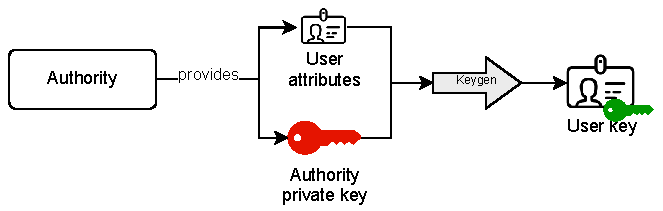
\includegraphics[width=\textwidth,height=0.7\textheight,keepaspectratio]{images/diagrams/keygen_diagram.pdf}
\end{figure}
\end{frame}

\begin{frame}
\frametitle{Encryption process}
\begin{itemize}
\item To encrypt data, a user provides the system with the data to be encrypted, together with an access policy.
\item The access policy is a boolean expression of attributes required to decrypt the data.
\item A random symmetric key is generated and used to encrypt the data with AES.
\item The same symmetric key is then encrypted using MA-ABE with the public keys of the authorities involved in the access policy.
\item Both the encrypted symmetric key and the encrypted data are returned to the user.
\end{itemize}
\end{frame}

\begin{frame}
\frametitle{Encryption Workflow Diagram}
\begin{figure}
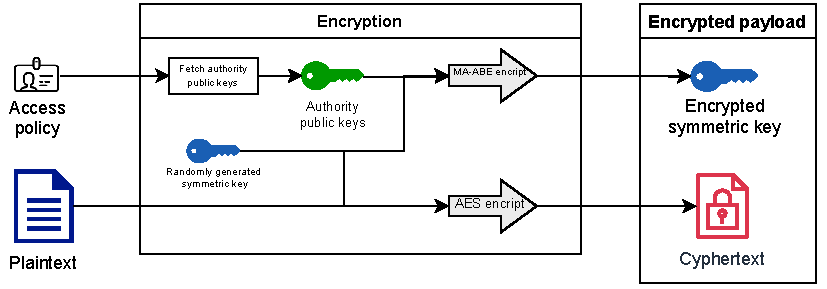
\includegraphics[width=\textwidth,height=0.7\textheight,keepaspectratio]{images/diagrams/encryption_diagram.pdf}
\end{figure}
\end{frame}

\begin{frame}
\frametitle{Decryption Process}
\begin{itemize}
\item To decrypt data, a user must possess a set of attribute keys that satisfies the access policy defined during encryption.
\item The process first decrypts the symmetric key using the MA-ABE keys provided by the user and then uses the symmetric key to decrypt the payload with AES.
\item This workflow enforces the access policy by requiring valid attribute keys to access the data.
\end{itemize}
\end{frame}

\begin{frame}
\frametitle{Decryption Workflow Diagram}
\begin{figure}
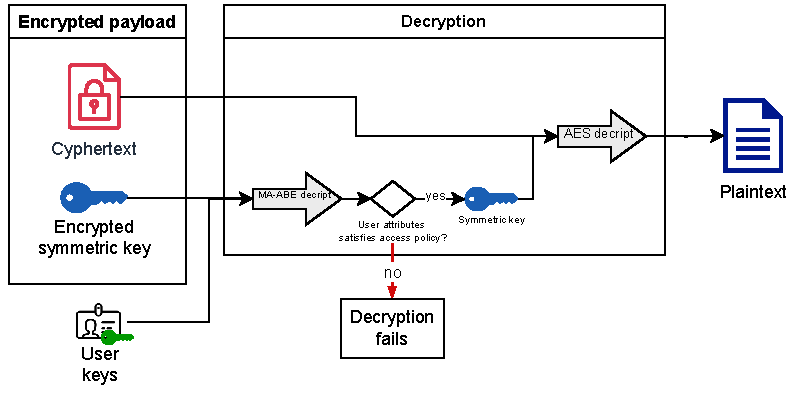
\includegraphics[width=\textwidth,height=0.7\textheight,keepaspectratio]{images/diagrams/decryption_diagram.pdf}
\end{figure}
\end{frame}

% --- Experimental Setup ---
\section{Experimental Setup}

\begin{frame}
\frametitle{Evaluation Strategy and Tools}
The evaluation aimed to measure performance, scalability, and cryptographic overhead.
\begin{itemize}
\item A RESTful API was developed to provide endpoints for all cryptographic operations.
\item \textbf{Locust} was used for load testing to simulate concurrent users.
\item \textbf{Gunicorn} managed concurrent requests with configurable workers and threads.
\item \textbf{Charm-Crypto} provided the implementation of the MaabeRW15 scheme for MA-ABE.
\item \textbf{Flask}, \textbf{Flask-RESTX} were used for API generation.
\item \textbf{Redis} was used for key storage and management.
\item All services were containerized with \textbf{Docker} for reproducibility.
\end{itemize}
\end{frame}

% --- Results and Discussion ---
\section{Results and Discussion}

\begin{frame}
\frametitle{Tests}
We tested system performance for a combination of variables:
\begin{itemize}
\item Threads and workers on the server.
\item Payload size.
\item Simultaneous user load.
\item Policy size.
\end{itemize}

We also measured the storage required for the user keys for different numbers of attributes.
\end{frame}

\begin{frame}
\frametitle{Concurrency Analysis}
\begin{itemize}
\item The system scales exponentially with the number of \textbf{processes (workers)} but does not benefit from multi-threading due to Python's Global Interpreter Lock (GIL).
\item From 5 workers onwards, the system performance stays stable, going from around 8.5 seconds to 200 milliseconds.
\item Due to those results and to Gunicorn recommendation (based on the number of processor cores in the test bed machine), we decided to proceed to the subsequent tests with 25 workers and 1 thread.
\end{itemize}
\end{frame}

\begin{frame}
\frametitle{Response time vs. number of workers}
\begin{figure}
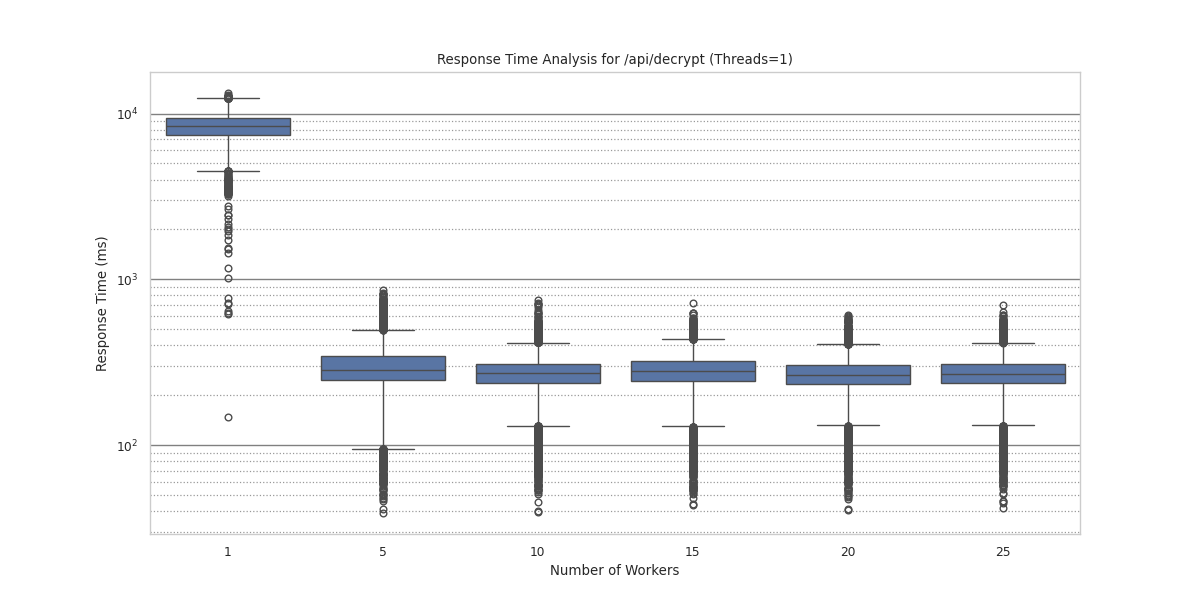
\includegraphics[width=\textwidth,height=0.7\textheight,keepaspectratio]{images/phase1/api_decrypt/response_time_threads_1.png}
\end{figure}
\end{frame}

\begin{frame}
\frametitle{Response time vs. number of threads}
\begin{figure}
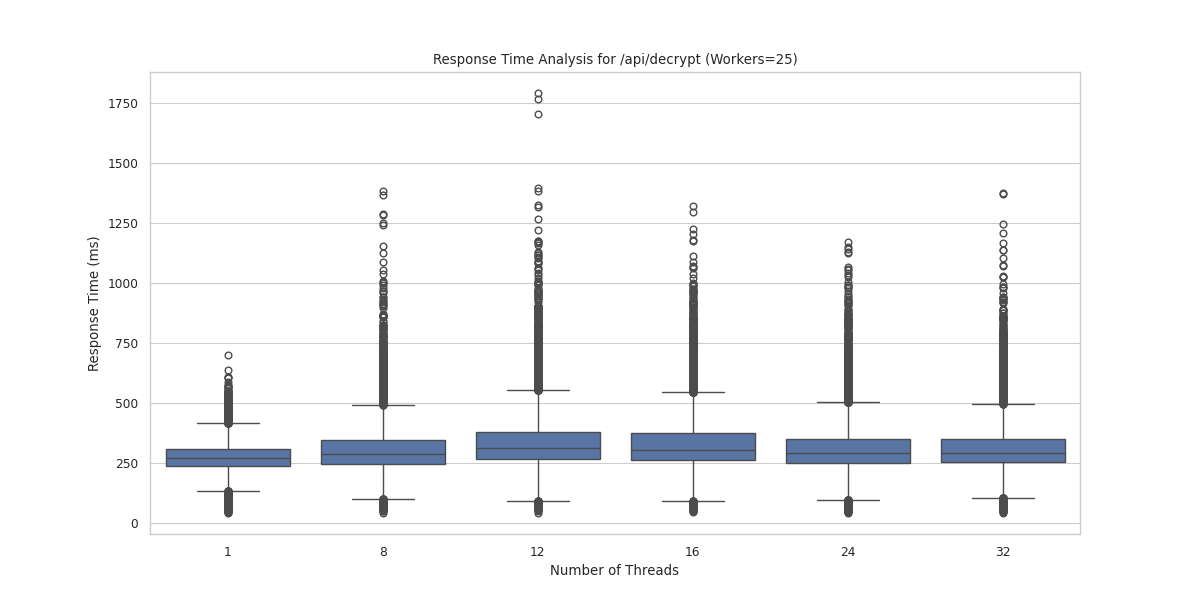
\includegraphics[width=\textwidth,height=0.7\textheight,keepaspectratio]{images/phase1/api_decrypt/response_time_workers_25.png}
\end{figure}
\end{frame}

\begin{frame}
\frametitle{Payload Size Impact}
\begin{itemize}
\item Response times increase linearly with larger payloads, with decryption times being significantly higher than encryption times due to the higher complexity of the operation.
\item This confirms the hybrid approach's suitability for large datasets, balancing security and performance.
\end{itemize}
\end{frame}

\begin{frame}
\frametitle{Encryption time vs. payload size}
\begin{figure}
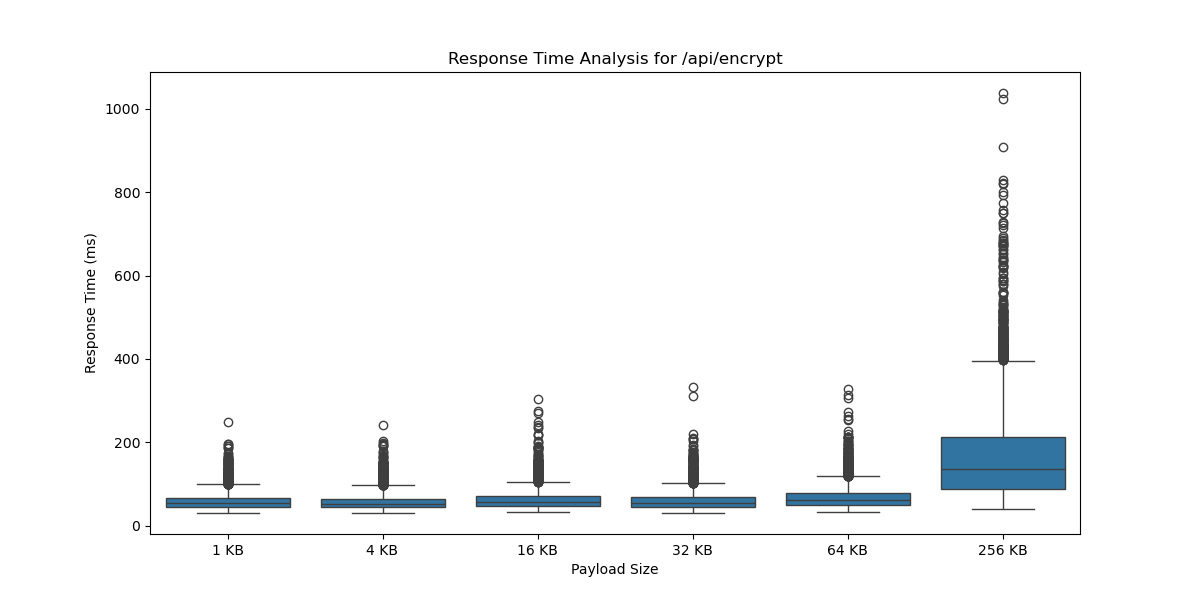
\includegraphics[width=\textwidth,height=0.7\textheight,keepaspectratio]{images/phase2/response_time_api_encrypt.png}
\end{figure}
\end{frame}

\begin{frame}
\frametitle{Decryption time vs. payload size}
\begin{figure}
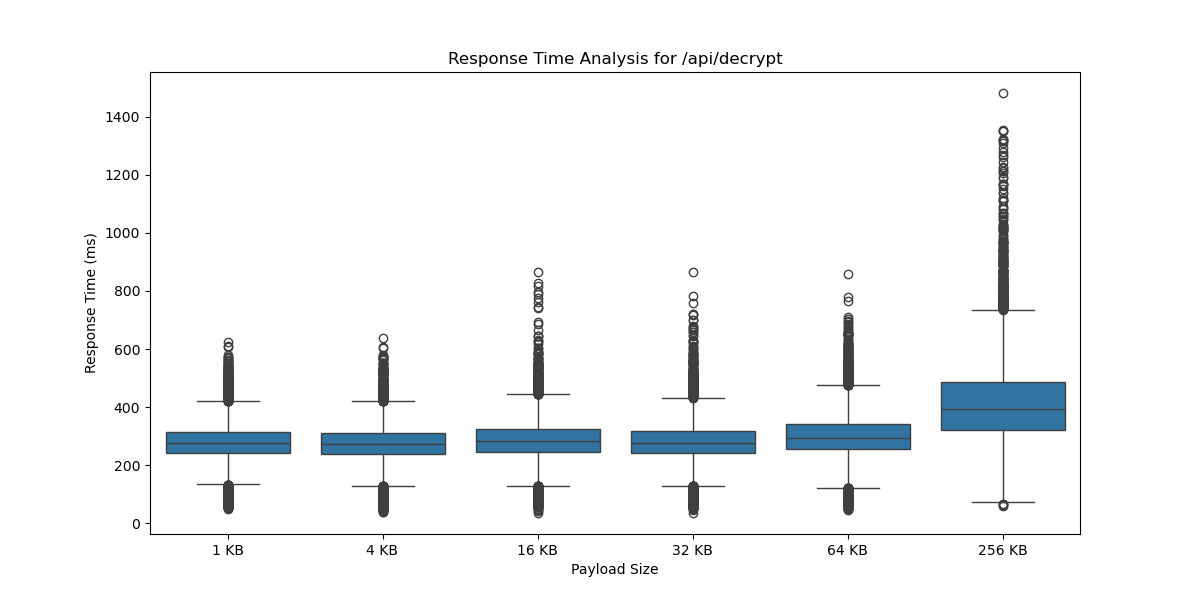
\includegraphics[width=\textwidth,height=0.7\textheight,keepaspectratio]{images/phase2/response_time_api_decrypt.png}
\end{figure}
\end{frame}

\begin{frame}
\frametitle{User Load Impact}
\begin{itemize}
\item The system handles moderate user loads well, with response times remaining stable up to 100 concurrent users.
\item Performance degrades at higher concurrency levels, indicating the need for further optimization or scaling strategies in high-demand scenarios.
\end{itemize}
\end{frame}

\begin{frame}
\frametitle{Response time vs. number of users}
\begin{figure}
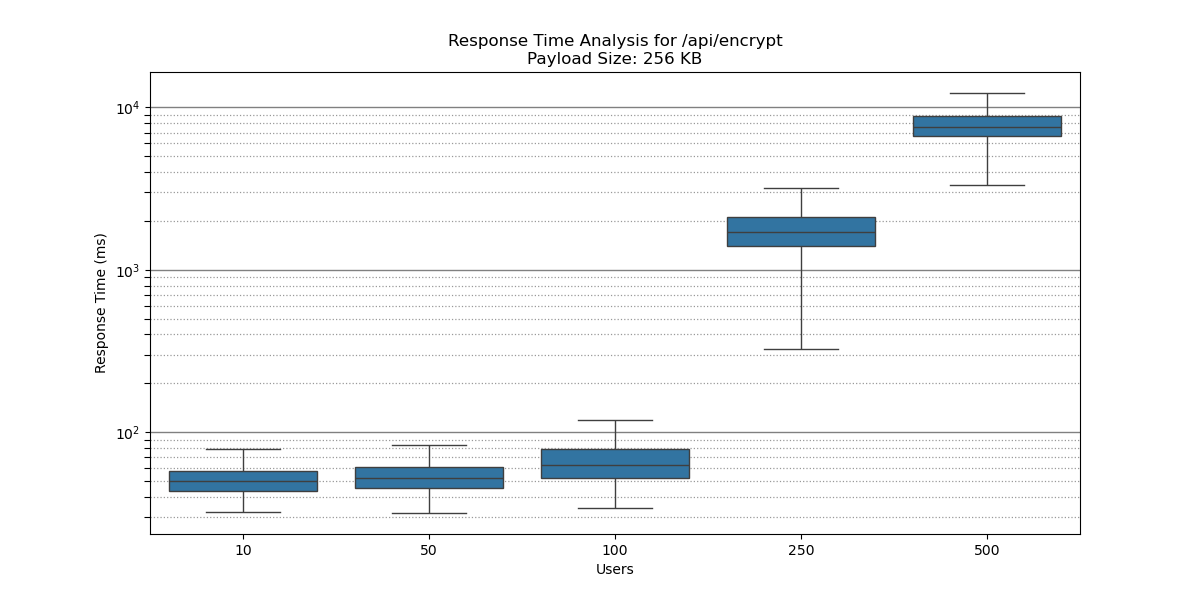
\includegraphics[width=\textwidth,height=0.7\textheight,keepaspectratio]{images/phase3/response_time_api_encrypt_256KB.png}
\end{figure}
\end{frame}

\begin{frame}
\frametitle{Impact of Policy Complexity}
\begin{itemize}
\item The complexity of the access policy (number of attributes) significantly affects decryption times, with more complex policies leading to longer response times.
\item This highlights the trade-off between security granularity and performance, as more attributes provide finer control but increase computational overhead.
\end{itemize}
\end{frame}

\begin{frame}
\frametitle{Decryption time vs. attributes}
\begin{figure}
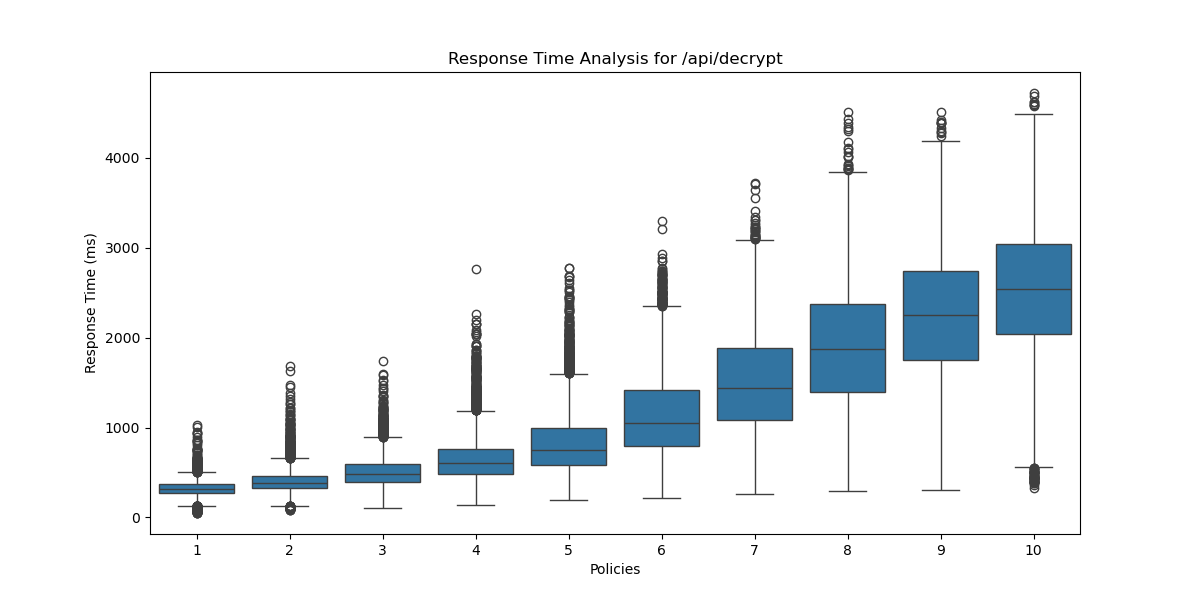
\includegraphics[width=\textwidth,height=0.7\textheight,keepaspectratio]{images/phase4/response_time_api_decrypt.png}
\end{figure}
\end{frame}

\begin{frame}
\frametitle{Impact of User Key Size}
\begin{itemize}
\item The size of the user keys increases linearly with the number of attributes, impacting storage requirements and potentially affecting performance.
\item This is a critical consideration for systems with many users or attributes, as larger keys can lead to increased I/O operations and slower response times.
\end{itemize}
\end{frame}

\begin{frame}
\frametitle{Key size vs. number of attributes}
\begin{figure}
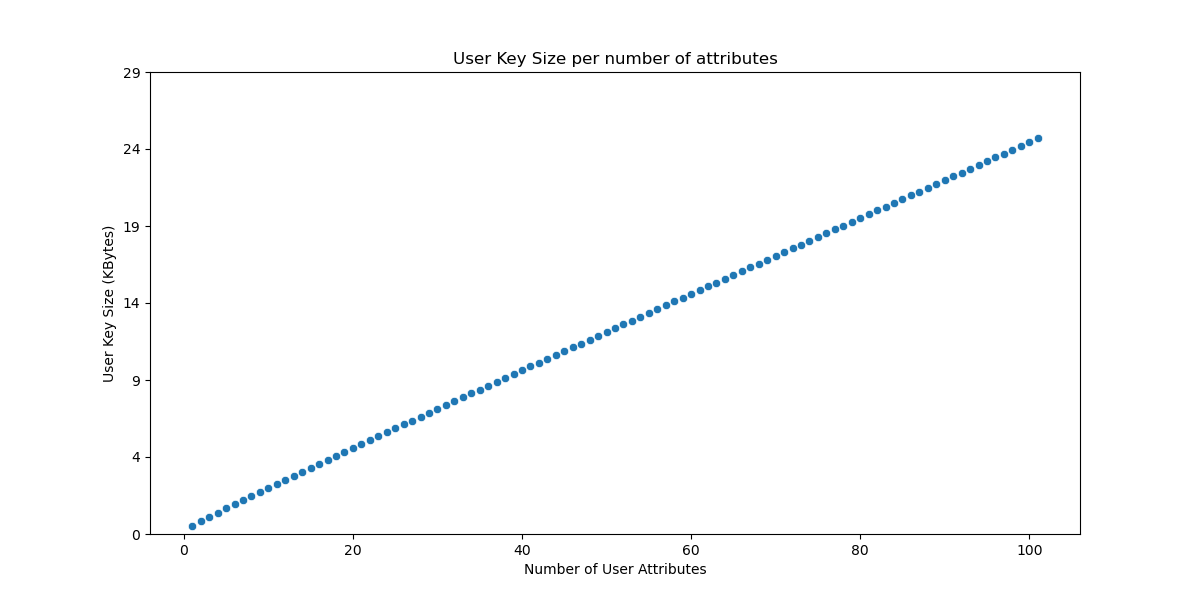
\includegraphics[width=\textwidth,height=0.7\textheight,keepaspectratio]{images/key_size_analysis/user_key_size_analysis.png}
\end{figure}
\end{frame}

% --- Conclusion ---
\section{Conclusion and Future Work}

\begin{frame}
\frametitle{Conclusion}
\begin{itemize}
\item This thesis successfully addressed a critical gap in HIoT data security by proposing, implementing, and evaluating a hybrid MA-ABE and AES cryptographic scheme.
\item The evaluation confirmed that the proposed solution is a viable and effective method for enforcing robust, fine-grained access control in decentralized HIoT systems.
\item The results highlight a practical trade-off between security granularity and performance, providing valuable insights for real-world deployment.
\end{itemize}
\end{frame}

\begin{frame}
\frametitle{Future Work}
\begin{itemize}
\item Full integration with the decentralized storage framework by \citeonline{laura2023} and end-to-end evaluation in a distributed environment.
\item Implementation of handling of binary data (e.g., medical images) directly, to reduce encoding overhead and improve efficiency.
\item Exploration of alternative key storage mechanisms to reduce I/O bottlenecks.
\item Investigation of further optimizations for MA-ABE operations, such as parallel processing or hardware acceleration.
\end{itemize}
\end{frame}

\begin{frame}[allowframebreaks]
\frametitle{References}
\bibliography{biblio}
\end{frame}

% --- Thank you ---
\begin{frame}
\frametitle{Thank you!}
\begin{center}
\Large Questions?
\end{center}
\vspace{2cm}
\InfContacts
\end{frame}

\end{document}